\chapter{Algorithms for Structural Variation Detection}\label{chap_related_work}

Recent publications have divided the majority of popular SV detection algorithms into four categories~\cite{Alkan:2011p547}. The first three categories depend upon first aligning short reads to the reference genome. Read pair (RP) based methods use the distance between and orientation of the mappings of the sequenced ends of DNA fragments to identify the signatures of SVs. Read depth (RD) approaches identify regions of the genome with anomalous raw numbers of mapped reads, which may indicate the presence of deletions or duplications (a category of SV's known as \emph{Copy Number Variations} (CNVs)). Split Read (SR) approaches attempt to find local mappings of portions of individual reads that span SV breakpoints. Finally, assembly-based methods attempt to construct as much of the genome sequence as possible directly from the reads, without first mapping them to the reference genome. The constructed sequence is then compared to the reference to identify SVs. Beyond these four categories, several recent approaches have attempted to integrate more than one type of signal to increase accuracy. 

\section{Read Pair Approaches}\label{section_read_pair}

Most read pair approaches begin by separating paired end mappings onto the reference genome into those that are \emph{concordant} and those that are \emph{discordant}. Discordant mappings deviate from the expected insert size or orientation of the fragment. These approaches then cluster the discordant mappings to find SVs with support from multiple discordantly mapped read pairs. Many of these approaches use only reads that are unambiguously mapped to the reference genome; this has the advantage of using the same set of alignments that are used for calling SNVs and indels in most sequencing pipelines. The BreakDancerMax component of BreakDancer~\cite{Chen:2009p3} is probably the most widely used of these algorithms. BreakDancer looks for regions of the genome that anchor more anomalous read pairs than expected according to its model; if two of these regions are connected by a minimum number of discordant read pairs, it calls an SV that links them. GASV~\cite{Sindi:2009gu}, PEMer~\cite{Korbel:2009dy}, and SVDetect~\cite{Zeitouni:2010p8} all operate on similar principles, differing primarily in the method used to cluster discordant read pairs that support the same potential SV call.

\begin{figure}
\centering
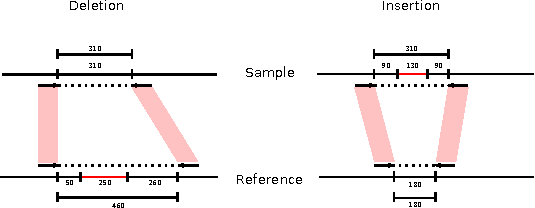
\includegraphics[width=\textwidth]{figures/rp_signatures.pdf}
\caption{Detecting deletions and insertions from the distance between mappings of paired reads. For the case of a deletion, a fragment with a 310bp internal insert size is created from the sample DNA, in a region in which 250bp has beeen deleted relative to the reference. The two reads when mapped to the reference will be 460bp apart, providing evidence for a deletion if we expect the internal insert size to be approximately 300bp. A 310bp internal insert size fragment that overlaps a 150bp insertion in the sample, conversely, will give a distance between reads of 180bp when mapped to the reference.}
\label{rp_signatures}
\end{figure}

\begin{figure}
\centering
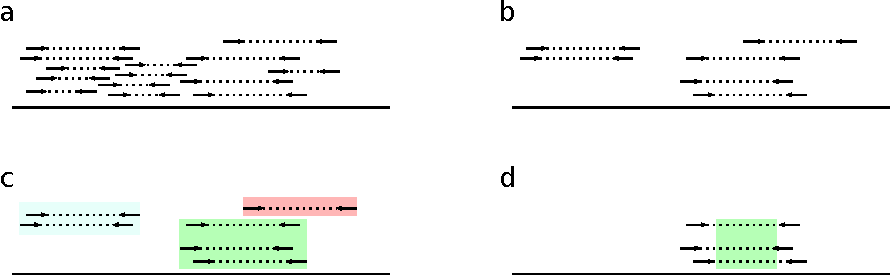
\includegraphics[width=\textwidth]{figures/rp_method_workflow.pdf}
\caption{The general algorithmic steps of a classic read-pair algorithm. a) The algorithm accepts a set of alignments of paired reads to the reference as input. b) The algorithm identifies discordant read pairs. c) Discordant pairs are clustered to find groups that could support the same algorithm. d) Clusters of discordant read pairs are filtered (in this case, by the number of supporting read pairs), and bounds on the potential breakpoints are identified.}
\label{rm_method_workflow}
\end{figure}

A second group of RP methods attempt to include discordant read pairs which cannot be unambiguously mapped to the reference genome in their analysis, in an effort to improve sensitivity in repetitive regions of the genome. One approach to incorporating this type of information can be found in \emph{soft clustering} algorithms, which assign each ambiguously mapped read pair to one of its mappings such that it clusters with other discordant read pairs. These approaches include VariationHunter~\cite{Hormozdiari:2009p284}, which allocates ambiguously mapped reads by optimizing to a maximum parsimony explanation of all discordant reads; HYDRA~\cite{Quinlan:2010gf}, which takes a similar approach based on heuristics, and GASVPro~\cite{Sindi:2012kk}, which uses a Markov-Chain Monte Carlo sampling strategy to assign a read to its correct mapping. Even so, however, most methods use only a limited number of ambiguous discordant mappings per read pair, in part because of the storage and computational requirements necessary to process all or most ambiguous mappings of each read pair in a high-coverage data set.

Finally, CLEVER~\cite{Marschall:2012ek} took an alternative approach and showed that rather than classifying pairs as concordant or discordant and considering only those that are discordant, considering the distribution of all insert sizes allows the detection of smaller events. 

Read pair approaches have the advantage of being theoretically able to detect any type of SV except for multiple copy number duplications. Their disadvantages stem from the fact that they depend on comparing mapping distances between reads to the unknown size of the fragments from which they came. This means that they cannot capture the breakpoints of SVs with single nucleotide resolution, and that they depend on having a sequencing library with a tight distribution of fragment sizes in order to have power.

\section{Read Depth Approaches}

Read-depth (RD) approaches consider the changing depth of coverage of concordantly mapped reads along the genome to infer the presence of SVs. For example, a homozygously deleted region will have zero coverage in the reference genome, while a region that has been duplicated many times, as can happen in some regions of the genome and in some cancers, will have a much higher coverage than average. These approaches differ mainly in the statistical and signal processing techniques used to identify anomalous regions. For example, CNVnator~\cite{Abyzov:2011bk} uses a mean-shift approach to segment the genome into CNV regions. Other approaches in this category include MrFAST~\cite{Alkan:2009cr}, Event-Wise Testing~\cite{Yoon:2009kb}, and SegSeq~\cite{Chiang:2009di}.

RD approaches are good at finding large deletions and duplications. As previously noted, they are the only approach that can identify segments of the genome that have been duplicated multiple times. Their disadvantages are their lack of ability to reliably detect smaller events, and their breakpoint resolution, which is even lower than than of RP approaches.

\section{Split Read Approaches}

Split-read (SR) methods look for breakpoints within individual reads by mapping portions of the read to different genomic locations. Due to the computational challenge involved in aligning reads to the reference genome while allowing for very large gaps between portions of the read, they use different strategies to guide the search. Pindel~\cite{Ye:2009p2} looks for paired reads in which one read in the pair aligned to the reference genome but the other did not. Supposing that the other read may contain a breakpoint, it searches the reference nearby for split read mappings. CREST~\cite{Wang:2011p1607} takes advantage of aligners that insert gaps at the ends of read alignments when there are many mismatches between the read and the reference, known as \emph{soft clipping}. By looking for multiple alignments with soft clips at the same reference coordinate, it can identify breakpoints. 

Split read approaches can identify SVs with high specificity and single base breakpoint accuracy. They are particularly good at detecting smaller variants. However, their sensitivity is limited by coverage and the length of the reads. As read lengths increase with advances in sequencing technology, they will play a larger role in SV detection.

\section{Assembly-Based Approaches}

An alternative approach to mapping reads to the species reference to discover variants is to first attempt to directly assemble the genomic sequence from which the reads were generated (AS approaches). This typically involves the construction of a \emph{de Bruijn} graph to represent the overlapping k-mers in the entire read set, and then walking the graph to construct the longest possible unambiguous sequence of k-mers. Although most work in assembly is focused on \emph{de novo} assembly, when there is no reference for the organism being sequenced, one approach that is targeted at detecting SV's, among other goals, is Cortex~\cite{Iqbal:2012p1837}. Cortex uses the reference to guide assembly with a colored de Bruijn graph structure, and can therefore identify SVs by walking colored paths in its graph.

While AS approaches can theoretically identify any type of SV, in practice assembly requires extremely high coverage (typically 100X). In addition, the computational requirements necessitate high-memory servers, making the task difficult to run on widely available, non-specialized hardware. Finally, genome assembly using short reads tends to collapse identical repeats, leading to a loss of visibililty in repetitive regions of the genome and in segmental duplications\cite{Alkan:2011hs}. Because SVs are enriched in these repetitive regions, this could potentially lead to many false negative calls, and potentially even false positives if repetitive regions are assembled incorrectly, as a loss of a set of repeats could look like a deletion.

\section{Hybrid Approaches}

Recently, approaches have started to appear that try to combine multiple signals in order to improve accuracy. These fall into two groups: those that independently execute more than one of the basic approaches described above and then integrate the results, and those that explicitly create new algorithms to process multiple signals simultaneously.

\subsection{Pipelines}

Pipelines such as SVMerge~\cite{Wong:2010p1271} and HugeSeq~\cite{Lam:2012jy} independently execute multiple algorithms of different types and then attempt to merge the results together. PeSV-Fisher~\cite{Escaramis:2013dm} implements classical RP and RD approaches and then integrates and filters the results. While the integration of these approaches could detect any type of variant detectable by any individual algorithm, it is difficult to combine results from different approaches in a principled manner, and the large number of dependencies and complex parameterization and configuration required has prevented adoption of these pipelines outside of the laboratories in which they were created.

\subsection{Modified Basic Algorithms}

Other tools use one of the four principle approaches outlined above, but have incorporated other signals into their algorithms to improve accuracy. GASVPro~\cite{Sindi:2012kk} is primarily an RP based method, but it used RD signals to validate its predicted breakpoints, assuming that coverage directly around the breakpoint, and in predicted deleted regions, should be reduced. DELLY~\cite{Rausch:2012he} and PRISM~\cite{Jiang:2012cp}, meanwhile, use RP based approaches to identify candidate SV regions, and then guide an SR search for the exact breakpoints of those SVs. Typically, these modifications seem to improve specificity at the expense of sensitivity.

\subsection{Mixtures of Distributions}\label{section_mixture_of_distributions}

Another class of hybrid solution explicitly models the expected number of concordant and discordant pairs at normal and variant locations, effectively combining RP and RD strategies. MoDIL~\cite{Lee:2009da} and the BreakDancerMini component of BreakDancer~\cite{Chen:2009p3} model the distribution of insert sizes at candidate locations in the genome using a Gaussian mixture model. This has two advantages: because reads are not categorized as concordant or discordant based on a hard threshold, it is possible to detect smaller insertions and deletions; and these approaches can explicitly model the zygosity (presence of the variant on one or both of the pairs of chromosomes in the cell) of the variant in the sample, and potentially classify the variant as homozygous or heterozygous. The disadvantage of this approach in these implementations has been the computational requirements, although as we shall see, this strategy lends itself to parallelization. SVMiner~\cite{Hayes:2012ia} follows a somewhat similar approach but does not explicitly model the distribution of insert sizes of read pairs; rather, it created feature vectors based on the number of concordant and discordant read pairs at each locus for deletions, or the number of pairs in each orientation for inversions, and fits a mixture model to the observed distribution of feature vectors across all candidate SVs.

\section{Development of an SV Detection Pipeline for a Cancer Dataset}\label{section_aml_pipeline}

\subsection{Preparation of the Library}

Peripheral blood was collected from a patient with acute myelomonocytic leukemia (previously designated acute myeloid leukemia FAB M4) under a written and oral informed consent process reviewed and approved by the Institutional Review Board of Oregon Health \& Science University. Known cytogenetic abnormalities associated with this specimen included trisomy 8 and internal tandem duplications within the FLT3 gene. Mononuclear cells were separated on a Ficoll gradient, followed by red cell lysis. Mononuclear cells were immunostained using antibodies specific for CD3, CD14, CD34, and CD117 (all from BD Biosciences) and cell fractions were sorted using a BD FACSAria flow cytometer. Cell fractions isolated included T-cells (CD3-positive), malignant monocytes (CD14-positive), and malignant blasts (CD34, CD117-positive). We sequenced CD14+ cells on an Illumina Genome Analyzer II, producing 128,819,200 paired-end reads.

\subsection{Validation of AML Deletions by PCR}

Deletions identified in the AML dataset were validated by PCR. SVs to validate were selected based on calls made by BreakDancer, relying on the score and the number of the reads supporting each single event. Appropriate primers were designed with an internet-based interface, Primer3 \cite{Untergasser01082012}, considering the chromosome localization and orientation of the interval involved in the candidate rearrangement. The primers were checked for specificity using the BLAT tool of the UCSC Human Genome Browser \cite{Kent01042002}. All the primer pairs were preliminarily tested on the patient genomic DNA and a normal genomic DNA as control. The PCR conditions were as follows: 2 min at 95\degree C followed by 35 cycles of 30 sec at 95\degree C, 20 sec at 60\degree C, and 2 min at 72\degree C. All the obtained PCR products were sequenced and analyzed by BLAT for sequence specificity. 

\subsection{Results}

The variants identified include deletions in the gene CTDSPL/RBPS3, an AML tumor suppressor~\cite{Zheng:2012kk}, and NBEAL1, a gene up-regulated in some cancers~\cite{Chen:2004jo}. We are currently investigating these deletions to determine their functional impact on this patient. 